\documentclass{standalone}
    
    \usepackage{standalone}
    \usepackage{tikz}
    \usetikzlibrary{er,positioning, calc}
    
    \begin{document}%
        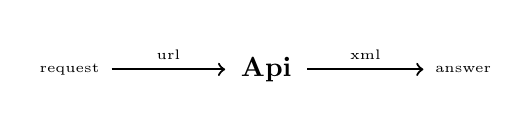
\begin{tikzpicture}%
            \tikzstyle{state}=[minimum width=0.8cm, font=\boldmath];%
            \node[circle] (0) at (0, 0) [state] {\tiny{request}};
            \node[circle] (1) at (2.5, 0) [state] {\textbf{Api}};
            \draw (0) edge[out=0, in=180, ->, thick] node [above] {\tiny{url}} (1);

            \node[circle] (2) at (5, 0) [state] {\tiny{answer}};
            \draw (1) edge[out=0, in=180, ->, thick] node [above] {\tiny{xml}} (2);
        \end{tikzpicture}
    \end{document}